% ============================================================================
%  main.tex --- Analysis of the "penguins" dataset
%
%  Encoding convention: accented characters are written with escape
%  sequences (e.g. \'a, \~n, \"u) so the source file is portable across
%  editors and does not depend on the file encoding.
% ============================================================================

\documentclass[11pt, a4paper]{article}

% --- Encoding and language --------------------------------------------------
% inputenc is omitted: modern LaTeX distributions default to UTF-8 and the
% escape sequences used for accents compile regardless of the file encoding.
\usepackage[T1]{fontenc}
\usepackage[english]{babel}
\usepackage{csquotes}

% --- Page layout ------------------------------------------------------------
\usepackage[a4paper, margin=2.5cm]{geometry}
\usepackage{fancyhdr}
\pagestyle{fancy}
\fancyhf{}
\fancyhead[L]{\small Analysis of the \texttt{penguins} dataset}
\fancyhead[R]{\small\thepage}
\renewcommand{\headrulewidth}{0.4pt}

% --- Math -------------------------------------------------------------------
\usepackage{amsmath}
\usepackage{amssymb}

% --- Graphics and tables ----------------------------------------------------
\usepackage{graphicx}
\usepackage{booktabs}
\usepackage{array}
\graphicspath{{images/}}

% --- Hyperlinks -------------------------------------------------------------
\usepackage[hidelinks]{hyperref}

% --- Abstract environment ---------------------------------------------------
% Redefines the default abstract to a compact centered block that also
% appears in the table of contents.
\renewenvironment{abstract}
{\clearpage\small\begin{center}\bfseries Abstract\end{center}\quotation}
{\endquotation\clearpage}

% --- Report metadata --------------------------------------------------------
\newcommand{\reportTitle}{Analysis of the ``penguins'' Dataset}
\newcommand{\reportSubtitle}{The Contribution of Sex over Physical Traits}
\newcommand{\reportAuthor}{Rub\'en Arellano}
\newcommand{\reportDate}{2025}
\newcommand{\reportRepo}{\url{https://github.com/RAAP276/Penguins-Analysis}}

% ============================================================================
\begin{document}
	
	\begin{titlepage}
	\centering
	\vspace*{2.5cm}
	
	{\Huge\bfseries \reportTitle \par}
	\vspace{0.8cm}
	{\Large\itshape \reportSubtitle \par}
	
	\vspace{3cm}
	{\large \reportAuthor \par}
	
	\vfill
	
	{\large \reportDate \par}
	\vspace{0.3cm}
	{\small \reportRepo \par}
\end{titlepage}
	
	% sections/abstract.tex
\begin{abstract}
	Penguins from the Palmer Archipelago differ in shape and size across species, and males and females differ systematically within each species. This report measures how much of a species or a body mass prediction can be recovered from physical traits alone, and how much the addition of sex improves it. Four models are compared on the \texttt{seaborn} \texttt{penguins} dataset: logistic regression and a decision tree for classification, and linear regression and a random forest for regression. Each model is trained under two feature configurations, one using only the four continuous physical traits and one adding sex. To separate the effect of sex from the effect of the particular training sample, the training data is split into two disjoint halves that share the same test set, and every configuration is evaluated under both halves. Logistic regression gains between 0.045 and 0.060 in accuracy when sex is added, and the two regressors gain between 0.048 and 0.075 in R\textsuperscript{2}. The sign of the gain is the same across both training subsets in every case, which supports the conclusion that the effect is real and not an artifact of a particular random split. The decision tree is the only model with no measurable gain, consistent with its ability to recover size-related splits directly from the physical traits. The main limitations are the small test set, a leakage in the scaler fit, and the absence of a depth constraint on the tree.
\end{abstract}
\addcontentsline{toc}{section}{Abstract}
	
	\clearpage
	\tableofcontents
	\clearpage
	
	\section{Introduction}
\label{sec:introduction}

The \texttt{penguins} dataset ships with the \texttt{seaborn} library and contains morphological measurements of 344 adult penguins from three species (\textit{Adelie}, \textit{Chinstrap} and \textit{Gentoo}) collected on three islands of the Palmer Archipelago. For each individual the dataset records four continuous physical traits (bill length, bill depth, flipper length and body mass) together with two categorical attributes: island of origin and sex. Species are strongly separated by morphology, which makes this dataset a common benchmark for classification. Males and females also differ systematically in size, which raises the question of how much a model gains from knowing sex.

This report answers two questions: the first is how well species can be predicted from physical traits alone and how much that changes when sex is added; the second is whether the same pattern holds when body mass is the regression target instead. Four supervised models are compared: logistic regression and a decision tree for classification, and linear regression and a random forest for regression. A repeated A/B design is used to check whether the conclusions depend on which rows end up in the training set.

The rest of the report is organized as follows. Section~\ref{sec:data_loading} covers data selection, loading and preprocessing. Section~\ref{sec:classification} and Section~\ref{sec:regression} present the classification and regression studies. Section~\ref{sec:robustness} checks whether the conclusions hold when the training set is split into two disjoint halves. Hyperparameter optimization of the decision tree is covered in Section~\ref{sec:hyperparameter_tuning}. Section~\ref{sec:conclusion} closes with the main findings.
	% sections/02_data_loading.tex
\section{Data Selection, Loading and Preprocessing}
\label{sec:data_loading}

Every supervised model depends on the data it is trained on. Before fitting anything, the dataset has to be selected, loaded and cleaned so that the predictors and the target are in a form the algorithms can consume. This section describes those steps: where the data come from, how missing values are handled, how categorical attributes are encoded and how the continuous traits are rescaled.

\subsection{Data selection and loading}

The dataset used in this report is the \texttt{penguins} DataFrame distributed with the \texttt{seaborn} library. It is loaded directly from the library, so no external file is downloaded or read from disk. The frame has 344 rows and 7 columns: the categorical target \texttt{species}, the categorical attribute \texttt{island}, four continuous physical traits (bill length, bill depth, flipper length and body mass) and the categorical attribute \texttt{sex}.

\subsection{Preprocessing}

The dataset is first inspected to count how many rows contain at least one missing value. There are 11 such rows out of 344, which is 3.2 \% of the data. That fraction is small enough to be discarded without meaningfully reducing the sample, so the rows are removed and the remaining 333 are kept.

The two categorical columns used by the models, \texttt{species} and \texttt{sex}, are then encoded as integers. Species are mapped to 1, 2 and 3 in the order Adelie, Chinstrap, Gentoo. Sex is mapped to 0 for males and 1 for females. Integer encoding is preferred over one-hot vectors to keep the feature representation compact and reduce the amount of input the models have to process.

The column \texttt{island} is not used. The study predicts species from physical traits of the individual, and island is not a physical trait. It is an environmental attribute that correlates strongly with species, so including it would leak information about the target.

The last step is to rescale the four continuous physical traits to the [0, 1] range using \texttt{MinMaxScaler}. Only those four columns are rescaled. Species and sex are labels, not magnitudes, so scaling them would be meaningless. The scaler is fitted once on the full cleaned frame and reused in every configuration of the study.
	% sections/03_classification.tex
\section{Classification}
\label{sec:classification}

Classification is the task of assigning each observation to one of a fixed set of categories. In this study the categories are the three penguin species, and the predictors are physical traits of the individual. Two models are compared, logistic regression and a decision tree. Each model is trained under two feature configurations: one using only the four continuous physical traits, and one adding the sex of the individual. Both configurations are trained on two disjoint training subsets that share the same test set, so that the effect of sex can be separated from the effect of the specific training rows. The design of those subsets is covered in Section~\ref{sec:robustness}; this section focuses on the models themselves and on the marginal contribution of sex.

The target variable is \texttt{species}. The features are bill length, bill depth, flipper length and body mass, and in the second configuration also sex. Both models are built with \texttt{scikit-learn}, use \texttt{random\_state=42} for reproducibility, are trained with the \texttt{fit} method, and produce predictions with the \texttt{predict} method.

\subsection{Logistic Regression}

Logistic regression is a linear model for classification. For each class it computes a linear combination of the predictors and passes the result through the logistic function, which produces a probability between 0 and 1. The predicted class is the one with the highest probability. Because the model is linear, its decision boundaries are hyperplanes in the feature space, an assumption that is restrictive in general but works well when the classes are well separated. The \texttt{scikit-learn} implementation applies L2 regularization by default, which helps control overfitting when the number of features is small.

\begin{figure}[htbp]
	\centering
	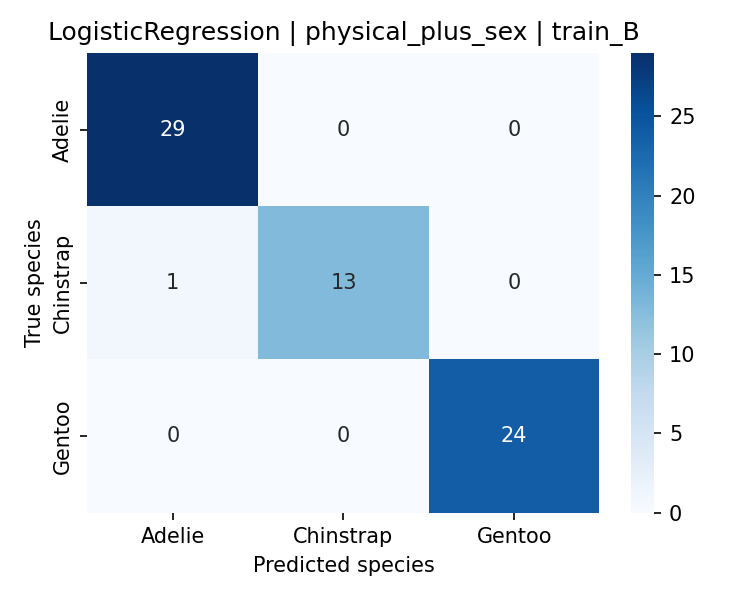
\includegraphics[width=0.7\textwidth]{figures/cm_LogisticRegression_physical_plus_sex_train_B.png}
	\caption{Confusion matrix for logistic regression with sex as a predictor, trained on subset B of the training data.}
	\label{fig:cm_logreg}
\end{figure}

On the shared test set, logistic regression with sex as a predictor reaches an accuracy of 0.985 and a weighted precision of 0.986 when trained on subset B, which is 66 correct predictions out of 67. The confusion matrix shows a single error: one Chinstrap individual is predicted as Adelie. Adelie and Gentoo are classified perfectly. The Chinstrap-Adelie confusion is consistent with the data alone, as the two species overlap in bill dimensions and are only separated cleanly by combining several traits.

\subsection{Decision Tree}

A decision tree partitions the feature space recursively. At each node it selects the feature and threshold that split the training data with the lowest impurity, measured by the Gini index. The process continues until the leaves are pure or a stopping criterion is met. Trees make no assumption about the shape of the decision boundary, so they can capture non-linear relations and interactions between predictors. The trade-off is that an unconstrained tree grows until it memorizes the training set, which is why hyperparameter tuning is needed. That step is covered in Section~\ref{sec:hyperparameter_tuning}.

\begin{figure}[htbp]
	\centering
	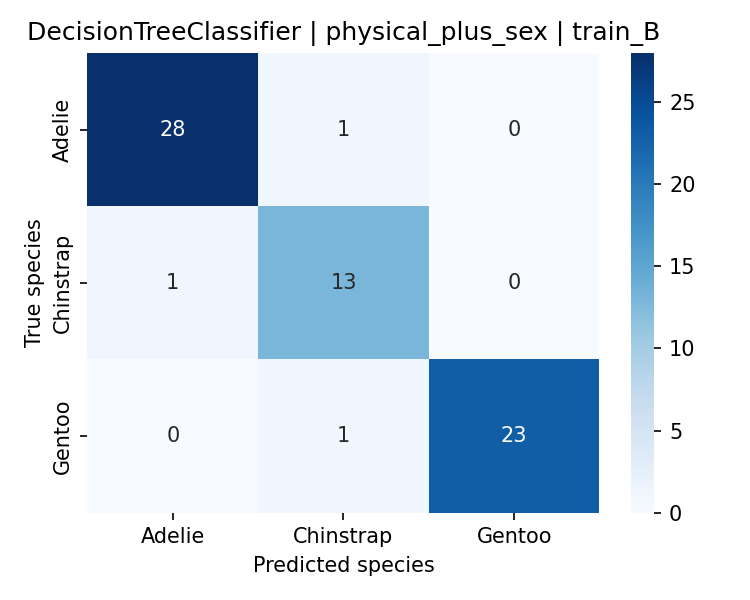
\includegraphics[width=0.7\textwidth]{figures/cm_DecisionTreeClassifier_physical_plus_sex_train_B.png}
	\caption{Confusion matrix for the decision tree with sex as a predictor, trained on subset B of the training data.}
	\label{fig:cm_tree}
\end{figure}

On the same test set, the decision tree with sex reaches an accuracy of 0.955 and a weighted precision of 0.955 when trained on subset B, which is 64 correct predictions out of 67. The confusion matrix shows three errors: one Adelie predicted as Chinstrap, one Chinstrap predicted as Adelie, and one Gentoo predicted as Chinstrap. The first two are consistent with the morphological overlap between Adelie and Chinstrap. The third is more surprising, since Gentoo is well separated from the other two species, and it reflects the tendency of an unconstrained tree to split the training data very finely and then generalize unevenly on a small test set.

\subsection{Effect of Sex on Classification}

Because each model is trained on two disjoint training subsets, the metrics vary slightly between runs. Table~\ref{tab:cls_metrics} reports the range of accuracy and weighted precision across the two subsets for each configuration.

\begin{table}[htbp]
	\centering
	\caption{Classification metrics on the shared test set. Ranges indicate the variation across the two disjoint training subsets.}
	\label{tab:cls_metrics}
	\begin{tabular}{lll}
		\toprule
		Model & Accuracy & Weighted precision \\
		\midrule
		Logistic regression (without sex) & 0.925 & 0.936 \\
		Logistic regression (with sex)    & 0.970 to 0.985 & 0.972 to 0.986 \\
		Decision tree (without sex)       & 0.910 to 0.955 & 0.914 to 0.957 \\
		Decision tree (with sex)          & 0.910 to 0.955 & 0.914 to 0.957 \\
		\bottomrule
	\end{tabular}
\end{table}

For logistic regression, adding sex raises accuracy by 0.045 on subset A and by 0.060 on subset B, which is the same as moving from 0.925 to 0.970 and from 0.925 to 0.985 respectively. The direction of the change is the same in both runs. For the decision tree, the metrics are indistinguishable on this test set with and without sex. This suggests that the splits selected by the tree already encode the information that sex provides, which is plausible given that male and female penguins differ mainly in body size, a variable the tree can split on directly.

The apparent gain in logistic regression raises a natural question: is it a real effect or a consequence of the particular training rows? Section~\ref{sec:robustness} addresses this by comparing the two subsets side by side.
	% sections/04_regression.tex
\section{Regression}
\label{sec:regression}

Regression is the task of predicting a continuous numerical value from a set of predictors. In this study the target is the body mass of the penguin, and the predictors are the other physical traits together with the species. Two models are compared, linear regression and a random forest. As in the classification study, each model is trained under two feature configurations, one using only physical traits and one adding sex, and both configurations are trained on the two disjoint training subsets that share the same test set. The design of those subsets is covered in Section~\ref{sec:robustness}.

The target variable is \texttt{body\_mass\_g}. The features are species, bill length, bill depth, flipper length and, in the second configuration, sex. Species is included as a predictor because it acts as a proxy for body size: Gentoo penguins are systematically larger than Chinstrap and Adelie, so the species label carries information about the target. All continuous features were previously rescaled to the [0, 1] range with MinMaxScaler, so the target and the error metrics are expressed in those normalized units, not in grams.

\subsection{Linear Regression}

Linear regression models the target as a linear combination of the predictors plus an intercept term. The coefficients are estimated by ordinary least squares, which minimizes the sum of squared residuals. The model is simple, fast, and easy to interpret, since each coefficient measures the change in the target associated with a unit change in one predictor while the others are held constant. Its main limitation is that it cannot capture non-linear relations or interactions between predictors unless those are added manually.

On the shared test set, linear regression with sex as a predictor reaches an R\textsuperscript{2} of 0.786 and an RMSE of 0.100 when trained on subset B. The R\textsuperscript{2} indicates that the model explains about 79 \% of the variance of the target in normalized units.

\subsection{Random Forest}

A random forest is an ensemble of decision trees. Each tree is trained on a bootstrap sample of the training data, and at each split only a random subset of the features is considered. The final prediction is the average of the individual tree predictions. This combination reduces the variance of a single tree and captures non-linear relations without requiring the user to specify them. The trade-off is that the model is harder to interpret than a single tree or a linear model, and training time grows with the number of trees.

On the same test set, the random forest with sex reaches an R\textsuperscript{2} of 0.841 and an RMSE of 0.086 when trained on subset B. It improves on linear regression on every metric, which is consistent with the presence of non-linear effects between body mass and the predictors.

\subsection{Effect of Sex on Regression}

Table~\ref{tab:reg_metrics} reports the range of R\textsuperscript{2} and RMSE across the two training subsets for each configuration and model.

\begin{table}[htbp]
	\centering
	\caption{Regression metrics on the shared test set. Ranges indicate the variation across the two disjoint training subsets.}
	\label{tab:reg_metrics}
	\begin{tabular}{lll}
		\toprule
		Model & R\textsuperscript{2} & RMSE \\
		\midrule
		Linear regression (without sex) & 0.711 to 0.712 & 0.116 to 0.117 \\
		Linear regression (with sex)    & 0.770 to 0.786 & 0.100 to 0.104 \\
		Random forest (without sex)     & 0.756 to 0.793 & 0.099 to 0.107 \\
		Random forest (with sex)        & 0.806 to 0.841 & 0.086 to 0.096 \\
		\bottomrule
	\end{tabular}
\end{table}

Adding sex improves both models on both training subsets. For linear regression the gain in R\textsuperscript{2} is between 0.058 and 0.075, and for the random forest it is between 0.048 and 0.050. The direction of the change is the same in all four runs, which is a stronger signal than in classification, where the decision tree showed no effect at all. The consistency makes sense from the modeling side: males and females differ systematically in body mass, so a variable that identifies sex provides information the physical traits cannot fully capture on their own.

Section~\ref{sec:robustness} compares the two training subsets side by side and discusses how much of this gain can be attributed to the specific rows used in each run.
	% sections/05_robustness.tex
\section{Robustness Check}
\label{sec:robustness}

The previous two sections showed that adding sex to the predictors improves species classification with logistic regression and body mass regression with both models. Those improvements could be a real effect of sex, or they could be an artifact of the particular rows that ended up in the training set. To distinguish the two cases, the training data is split into two disjoint halves and each model is trained twice, once on each half, always evaluated against the same test set.

\subsection{Design of the A/B Split}

The master train/test split is performed once, by row index, on the preprocessed frame. The test set is 20 \% of the rows and is stratified by species. The remaining 80 \% is partitioned into two disjoint halves of equal size, \texttt{train\_A} and \texttt{train\_B}, using a different random seed. The two halves are disjoint and their union equals the full training set. All feature configurations, all models and both studies use this same partition, so any difference between \texttt{train\_A} and \texttt{train\_B} comes from the training sample, not from a different test set or a different preprocessing step.

\subsection{Stability in Classification}

Table~\ref{tab:cls_stability} reports the accuracy of each classifier on the shared test set, for the two feature configurations and the two training subsets.

\begin{table}[htbp]
	\centering
	\caption{Classification accuracy across training subsets. The delta column is the change in accuracy when sex is added.}
	\label{tab:cls_stability}
	\begin{tabular}{llccc}
		\toprule
		Model & Subset & Without sex & With sex & Delta \\
		\midrule
		Logistic regression & train\_A & 0.925 & 0.970 & +0.045 \\
		Logistic regression & train\_B & 0.925 & 0.985 & +0.060 \\
		Decision tree       & train\_A & 0.910 & 0.910 & 0.000 \\
		Decision tree       & train\_B & 0.955 & 0.955 & 0.000 \\
		\bottomrule
	\end{tabular}
\end{table}

For logistic regression the delta is positive in both subsets, with a range of 0.045 to 0.060. The sign is the same in both runs, so the effect is stable with respect to the training sample. The magnitude varies, which is expected given that the test set has 67 rows and the standard error of an accuracy estimate at that size is close to 0.03. For the decision tree the delta is exactly zero in both subsets. The tree is not unstable, it is simply indifferent to sex: the splits it chooses already encode the information that sex provides.

\begin{figure}[htbp]
	\centering
	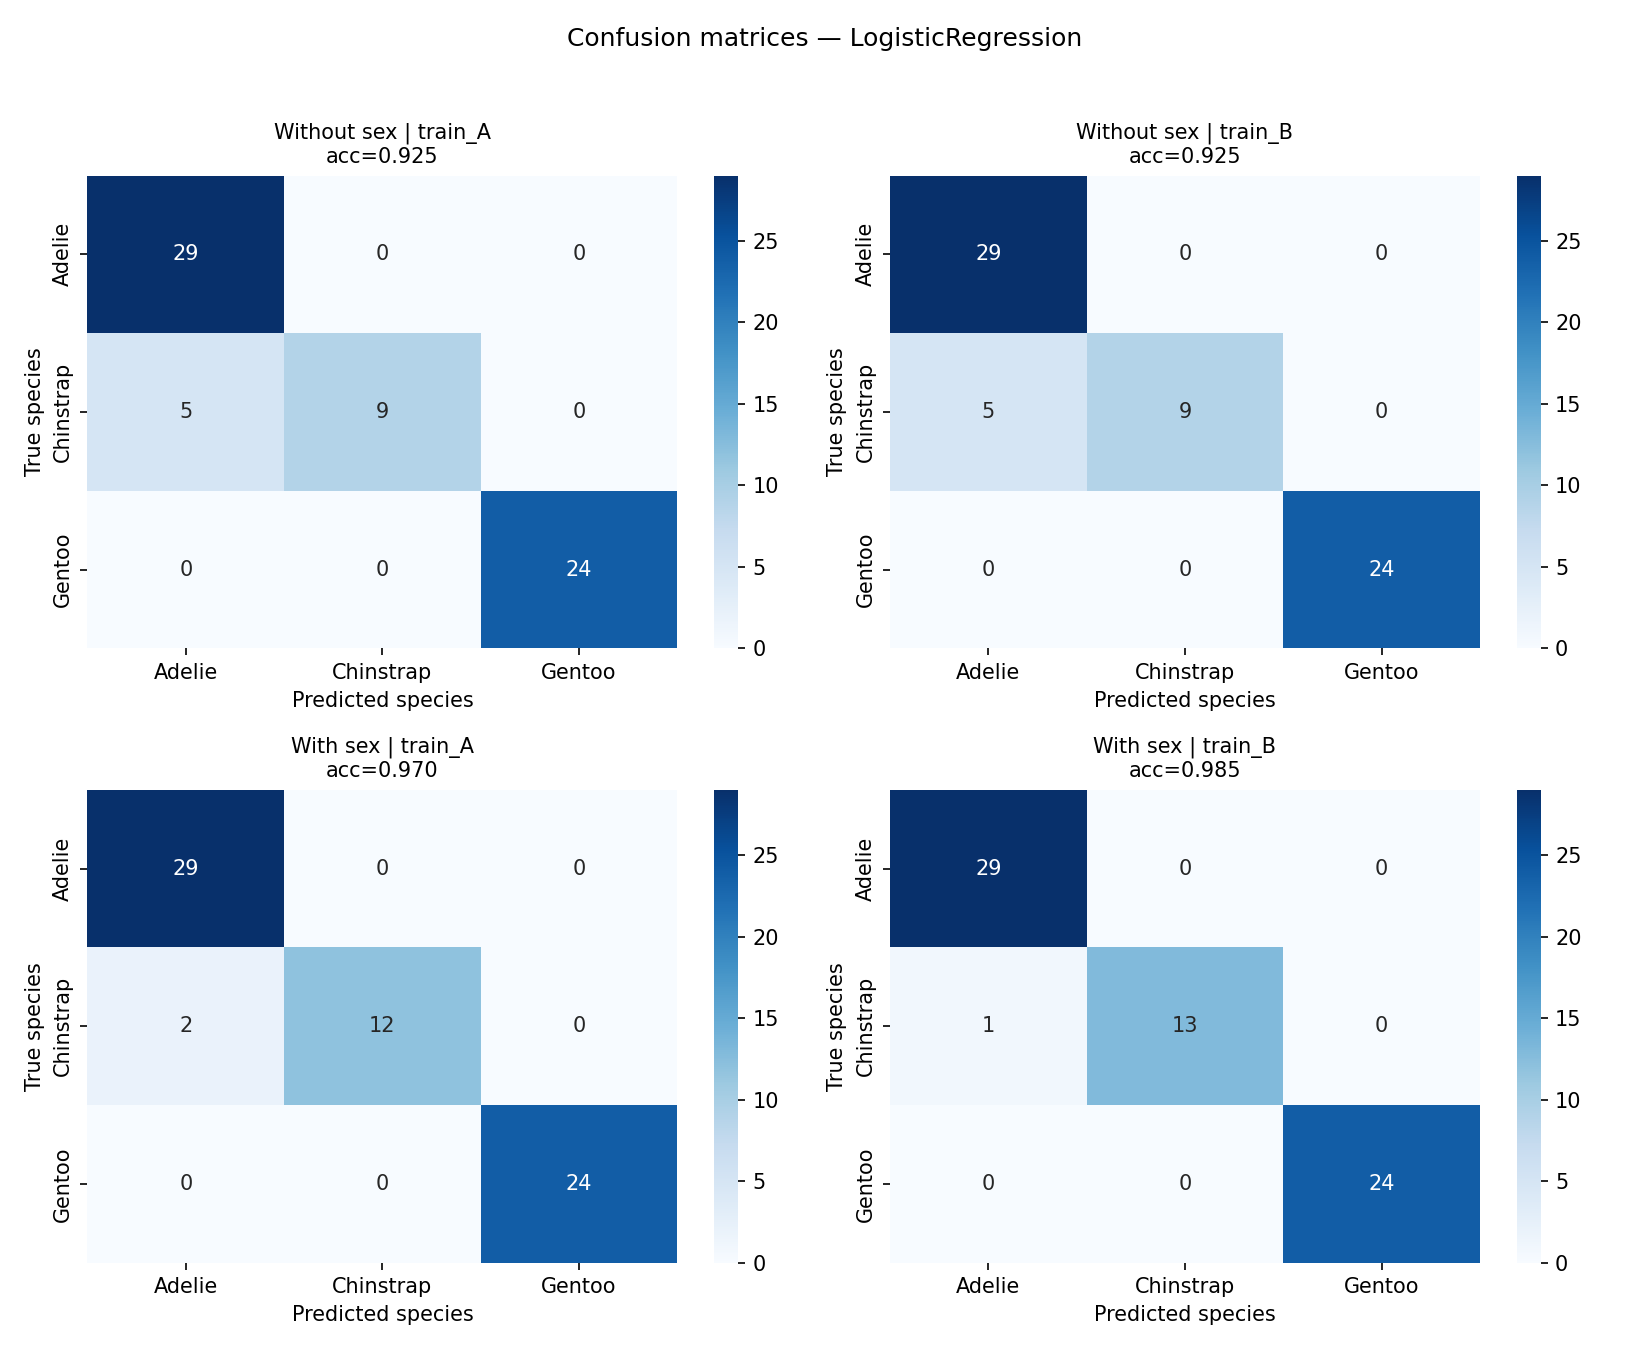
\includegraphics[width=0.95\textwidth]{figures/grid_LogisticRegression.png}
	\caption{Confusion matrices for logistic regression across feature configurations and training subsets.}
	\label{fig:grid_logreg}
\end{figure}

\begin{figure}[htbp]
	\centering
	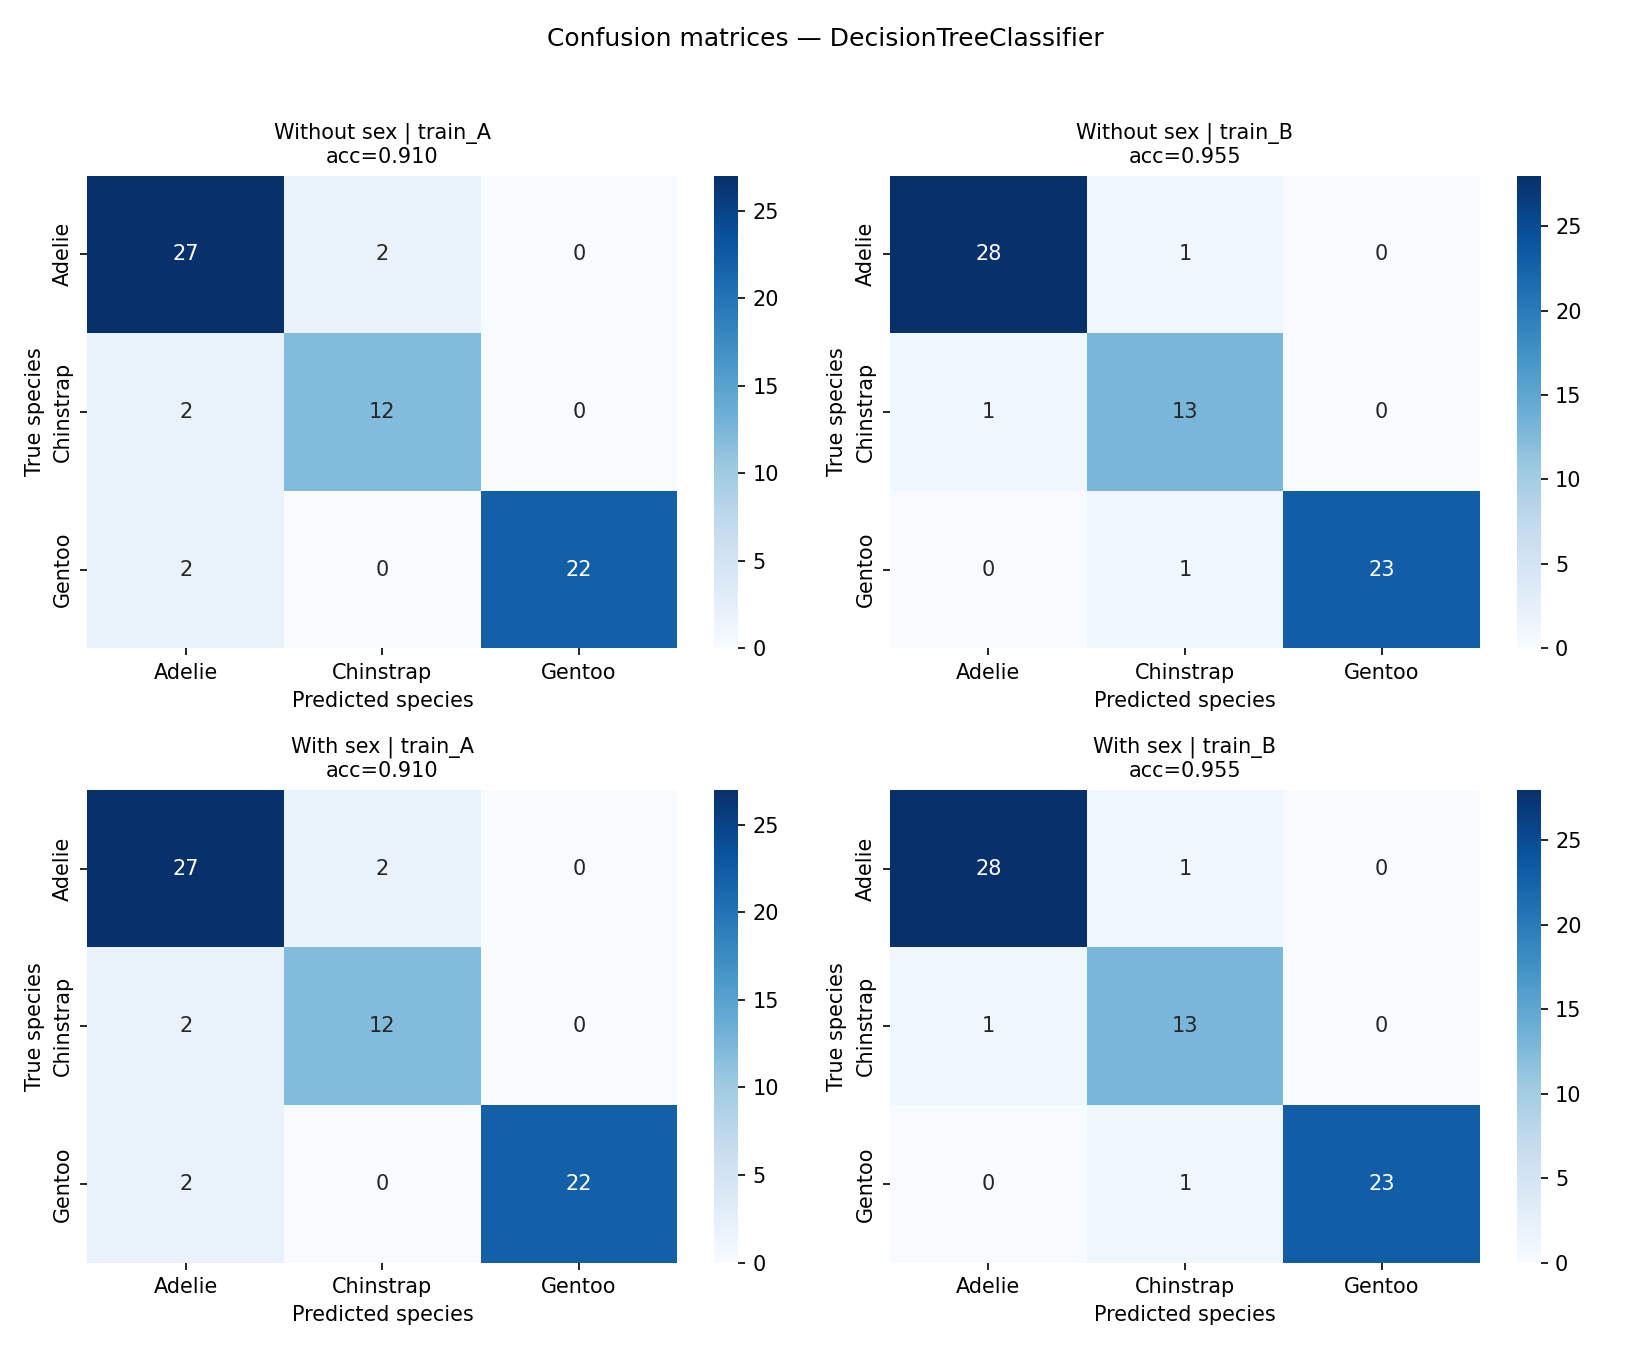
\includegraphics[width=0.95\textwidth]{figures/grid_DecisionTreeClassifier.png}
	\caption{Confusion matrices for the decision tree across feature configurations and training subsets.}
	\label{fig:grid_tree}
\end{figure}

\subsection{Stability in Regression}

Table~\ref{tab:reg_stability} reports R\textsuperscript{2} for each regressor on the shared test set, for the same four combinations.

\begin{table}[htbp]
	\centering
	\caption{Regression R\textsuperscript{2} across training subsets. The delta column is the change in R\textsuperscript{2} when sex is added.}
	\label{tab:reg_stability}
	\begin{tabular}{llccc}
		\toprule
		Model & Subset & Without sex & With sex & Delta \\
		\midrule
		Linear regression & train\_A & 0.712 & 0.770 & +0.058 \\
		Linear regression & train\_B & 0.711 & 0.786 & +0.075 \\
		Random forest     & train\_A & 0.756 & 0.806 & +0.050 \\
		Random forest     & train\_B & 0.793 & 0.841 & +0.048 \\
		\bottomrule
	\end{tabular}
\end{table}

For both regressors the delta is positive in both subsets, with ranges of 0.058 to 0.075 for linear regression and 0.048 to 0.050 for the random forest. The sign is consistent in all four runs, and the magnitude is also consistent for the random forest, which is a stronger signal than in classification. This matches the biological expectation: males and females differ systematically in body mass, and the sex variable provides information that the physical traits cannot fully recover on their own.

\subsection{Summary}

The A/B design isolates the effect of the training sample from the effect of the predictors. Across both studies, the sign of the effect of adding sex is the same in both training subsets, which supports the conclusion that the observed gains are real and not an artifact of a particular random split. The magnitude varies slightly between subsets, most likely because the test set is small, but the direction does not. The decision tree is the only case where sex has no measurable effect, and that is consistent with its ability to recover size-related splits directly from the physical traits.
	% sections/06_hyperparameter_tuning.tex
\section{Hyperparameter Optimization}
\label{sec:hyperparameter_tuning}

The decision tree in Section~\ref{sec:classification} was trained with the default parameters of \texttt{scikit-learn}, which means it grows until every leaf is pure or contains fewer samples than the minimum split size. On small datasets this behavior can lead to trees that fit the training data very closely and generalize poorly. Hyperparameter optimization is the process of searching for the combination of parameters that controls this growth and maximizes performance on unseen data.

The search was performed with \texttt{GridSearchCV} from \texttt{scikit-learn}. This method evaluates every combination of the values provided in a parameter grid using cross-validation on the training set and returns the combination with the best average score. Three parameters were explored.

\begin{itemize}
	\item \texttt{max\_depth}: the maximum depth of the tree. \texttt{None} allows nodes to expand until all leaves are pure or fall below \texttt{min\_samples\_split}. The values 5, 10 and 15 cap the depth and force the tree to stop earlier, which helps control overfitting.
	\item \texttt{min\_samples\_split}: the minimum number of samples required to split an internal node. Higher values prevent the tree from creating very small branches that only fit noise. The values explored were 2, 5 and 10.
	\item \texttt{min\_samples\_leaf}: the minimum number of samples allowed in a leaf node. Higher values force leaves to represent broader groups of samples. The values explored were 1, 2 and 4.
\end{itemize}

For each combination, a fresh \texttt{DecisionTreeClassifier} was trained and evaluated with 5-fold cross-validation on the training set. The metric used to select the best combination was accuracy. The search was run independently for each of the four branches of the study, that is, for each feature configuration (with and without sex) and each training subset (A and B).

\begin{table}[htbp]
	\centering
	\caption{Best hyperparameters selected by GridSearchCV for each branch.}
	\label{tab:tuning}
	\begin{tabular}{lllll}
		\toprule
		Configuration & Subset & \texttt{max\_depth} & \texttt{min\_samples\_split} & \texttt{min\_samples\_leaf} \\
		\midrule
		Without sex & train\_A & None & 2 & 1 \\
		Without sex & train\_B & None & 2 & 1 \\
		With sex    & train\_A & None & 2 & 1 \\
		With sex    & train\_B & None & 2 & 1 \\
		\bottomrule
	\end{tabular}
\end{table}

The same combination was selected in all four branches: \texttt{max\_depth=None}, \texttt{min\_samples\_split=2} and \texttt{min\_samples\_leaf=1}, which is exactly the default configuration of the classifier. This means that restricting the tree did not improve cross-validated accuracy on this dataset, and the unconstrained tree was already the best option under the metric used. The result is consistent with the fact that the penguins dataset is strongly separable: the tree does not need to overfit to achieve high accuracy, and its natural splits along physical traits already capture the structure of the classes.

Accuracy was chosen as the selection metric because the three species are roughly balanced after cleaning, so the metric does not hide poor performance on any single species. This is consistent with the per-class counts in the confusion matrices of Section~\ref{sec:classification}.
	% sections/07_conclusion.tex
\section{Conclusion}
\label{sec:conclusion}

This report compared four supervised models on the \texttt{penguins} dataset, two for classification and two for regression, and measured how much the sex of an individual adds to predictions based on physical traits alone. Both studies reached high performance on the test set. Logistic regression classified species with an accuracy of up to 0.985 and a weighted precision of 0.986, and the decision tree reached 0.955 on both metrics. For regression, the random forest predicted body mass with an R\textsuperscript{2} of up to 0.841, while linear regression reached 0.786. Hyperparameter optimization of the decision tree did not improve on the default configuration, which indicates that the tree was already well suited to this dataset under the metric used. The main finding is that adding sex to the predictors produces a consistent gain in every model where the effect is measurable: classification with logistic regression gained between 0.045 and 0.060 in accuracy, and regression gained between 0.048 and 0.075 in R\textsuperscript{2}, always with the same sign across two disjoint training subsets.

Three limitations should be considered when reading the results. First, the decision tree was left unconstrained in the final comparison. Although cross-validation selected the default parameters, an unlimited depth is a structural risk on datasets with more noise or less separation between classes, and a future iteration should test the same pipeline on such data. Second, the MinMaxScaler was fitted on the full cleaned frame before the train/test split. This is a methodological leakage: the scaler saw the test rows during fitting, which in this case has a small numerical effect but violates the rule that no information from the test set should influence training. The correct fix is to wrap the scaler and the model in a \texttt{Pipeline} from \texttt{scikit-learn} so that the scaler is refitted inside each fold. Third, the test set has only 67 rows. The standard error of an accuracy estimate at that size is close to 0.03, so the magnitudes of the reported gains should be treated as approximate. The sign of the effect of sex is stable across training subsets, which supports the qualitative conclusion, but the exact numbers may shift with a different random split.

The results of this study are reproducible. The pipeline uses a fixed random state, the A/B split is deterministic, and the notebooks and the report sources are versioned in a public repository. The approach can be extended to other datasets with the same structure, and the A/B design in particular is a low-cost way to check whether an observed effect is real or an artifact of the training sample.
	
\end{document}